% Generator: hand-authored TikZ schematic traced from source-visible edges and labels; projection is illustrative.
% Source ID: src-120ea104f8cb373f5731039fa9d36469df457869849f27420831962ef1ad2306
% PDF SHA-256: d0081500bd56d03199ddcf232fe8e870f2ecd7e9c41ba849417af9af79fbb702
% PDF page 1; printed page 124; question 17.
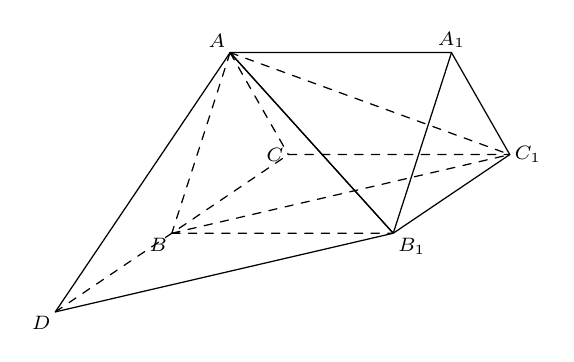
\begin{tikzpicture}[
  x=0.74cm,y=0.74cm,line width=0.45pt,line cap=round,line join=round,
  every node/.style={font=\scriptsize,inner sep=1.5pt}
]
  \coordinate (A)  at (0.7,4.2);
  \coordinate (A1) at (4.5,4.2);
  \coordinate (B)  at (-0.3,1.1);
  \coordinate (B1) at (3.5,1.1);
  \coordinate (C)  at (1.7,2.45);
  \coordinate (C1) at (5.5,2.45);
  \coordinate (D)  at (-2.3,-0.25);

  % Source-visible prism and auxiliary edges.
  \draw (D)--(A) (D)--(B1) (A)--(B1);
  \draw (A)--(A1)--(C1)--(B1)--cycle;
  \draw (A1)--(B1);
  \draw[dashed] (D)--(B)--(C) (A)--(B) (A)--(C);
  \draw[dashed] (A)--(C1) (B)--(B1) (B)--(C1) (C)--(C1);

  \node[above left] at (A) {$A$};
  \node[above] at (A1) {$A_1$};
  \node[below left] at (B) {$B$};
  \node[below right] at (B1) {$B_1$};
  \node[left] at (C) {$C$};
  \node[right] at (C1) {$C_1$};
  \node[below left] at (D) {$D$};
\end{tikzpicture}
